\documentclass[10pt,a4paper,fleqn,oneside]{book}
\usepackage[utf8]{inputenc}
\usepackage{graphicx}
\usepackage[italian]{babel}
\usepackage[margin=0.7in]{geometry}
\usepackage[colorlinks]{hyperref}
\usepackage[toc]{glossaries}
\usepackage{bookmark}
\usepackage{eurosym}
\usepackage[T1]{fontenc}
\usepackage{tabularx}
\usepackage{booktabs}
\usepackage[table]{xcolor}
\usepackage{enumitem}
\usepackage{makecell}


\title{Appunti di Economia}
\author{Andrea Franchini}

% TOC
\setcounter{tocdepth}{4}

% Paragraphs don't have indents
\setlength{\parindent}{3em}

% Reduce spacing between \items
\setlist[itemize]{noitemsep}

% Images
\graphicspath{ {./images/} }

% Lists have tiny bullet
\renewcommand\labelitemi{\textendash}
\renewcommand\labelitemii{\textendash}
\renewcommand\labelitemiii{\textendash}

% Pro e contro
\newcommand{\proandcons}[2]{
%    \begin{tabularx}{\linewidth}{>{\parskip1ex}X@{\kern4\tabcolsep}>{\parskip1ex}X}
    \begin{tabularx}{\linewidth}{>{\parskip1ex}X@{\kern4\tabcolsep}>{\parskip1ex}X}

        \toprule
        \hfil\bfseries Pro
        &
        \hfil\bfseries Contro
        \\\cmidrule(r{3\tabcolsep}){1-1}\cmidrule(l{-\tabcolsep}){2-2}
        
        %% PROS, seperated by empty line or \par
        #1

        &
        %% CONS, seperated by empty line or \par
        #2
        \\\bottomrule
    \end{tabularx}
}

% TextBox
\newcommand{\textbox}[1]{
\vspace{1em}
\begin{center}
    \begin{tabular}{|c|}
        \hline
        #1\\
        \hline
    \end{tabular}
\end{center}
}

% Highlight table row
\newcommand{\grayrow}{\rowcolor[gray]{.90}}

% Glossary
\makeglossaries

\newglossaryentry{imprenditore}{
    name=imprenditore,
    description={chi esercita professionalmente un'attività economica
    organizzata al fine della produzione o dello scambio di beni o di servizi}
}

\newglossaryentry{impresa}{
    name=impresa,
    description={attività economica organizzata, svolta professionalmente, al fine della
    produzione o dello scambio di beni o di servizi}
}

\newglossaryentry{lavsub}{
    name=lavoratore subordinato,
    description={chi si obbliga, mediante retribuzione a
    collaborare nell'\gls{impresa}, prestando il proprio lavoro, intellettuale o
    manuale, alle dipendenze e sotto la direzione dell'\gls{imprenditore}}
}

\newglossaryentry{societa}{
    name=società,
    description={contratto con cui \emph{due o più persone} conferiscono beni
    o servizi per l’esercizio in comune di un’attività economica allo scopo di
    dividerne gli \glspl{utile}}
}

\newglossaryentry{azienda}{
    name=azienda,
    description={\emph{complesso dei beni organizzati} dall'\gls{imprenditore} per
    l'esercizio dell'\gls{impresa}}
}

\newglossaryentry{ditta}{
    name=ditta,
    description={\emph{nome commerciale} scelto dall’imprenditore per
    esercitare l’\gls{impresa}: è un segno distintivo che consente ai consumatori di
    identificare l’impresa, ha valore commerciale e pertanto la legge ne garantisce
    l'\emph{uso esclusivo}}
}

\newglossaryentry{utile}{
    name=utile,
    description={indica la differenza tra ricavi e costi di un'impresa. Se tale
    differenza è positiva viene comunemente chiamato \emph{profitto}, in caso
    contrario viene chiamato perdita},
    plural=utili
}

\newglossaryentry{shareholder}{
    name=shareholder,
    description={I proprietari dell'impresa}
}

\newglossaryentry{stakeholder}{
    name=stakeholder,
    description={Insieme delle parti interessate (management, finanziatori a titolo oneroso,
    fornitori, clienti, dipendenti, organizzazioni sindacali, concorrenti, Stato}
}

\newglossaryentry{rischio}{
    name=rischio,
    description={impossibilità di prevedere con certezza gli esiti futuri delle 
    decisioni in merito alle attività dell’impresa (``probabilità di un evento
    e delle sue conseguenze'')}
}

\newglossaryentry{bizmodel}{
    name=business model,
    description={Il piano dell'impresa per creare, distrubuire e raccogliere
    valore}
}

\newglossaryentry{bizplan}{
    name=business plan,
    description={Il business plan è la descrizione dell’idea imprenditoriale in
    cui si dimostra che l’attività proposta merita fiducia più di altre
    possibilità di investimento}
}

\newglossaryentry{personagiuri}{
    name=personalità giuridica,
    description={un soggetto giuridico cui fanno capo diritti e doveri}
}

\newglossaryentry{formagiuri}{
    name=forma giuridica,
    description={la tipologia giuridica del soggetto a cui fa
    capo l’attività e le norme ad essa conseguenti}
}

\newglossaryentry{respill}{
    name=responsabilità illimitata,
    description={l’imprenditore (i soci) risponde (rispondono)
    delle perdite dell’impresa con tutto il suo (loro) patrimonio. Ad esempio,
    per pagare gli stipendi ai lavoratori l’imprenditore può essere
    costretto dal curatore fallimentare a vendere la propria abitazione}
}

\newglossaryentry{resplim}{
    name=responsabilità limitata,
    description={i soci rispondono delle perdite dell’impresa con i capitali
    conferiti nell’impresa. Il patrimonio personale dei soci (immobili, conti
    correnti bancari a loro intestati) non è intaccato dalle perdite dell’impresa}
}

\newglossaryentry{piccoloimpr}{
    name=piccolo imprenditore,
    description={``sono piccoli imprenditori coltivatori diretti del
    fondo, gli artigiani, i piccoli commercianti, coloro che esercitano un’attività
    professionale organizzata prevalentemente con il lavoro proprio e dei
    componenti della famiglia''}
}

\newglossaryentry{contabilita}{
    name=contabilità,
    description={Processo di individuazione, misurazione, analisi, interpretazione,
    comunicazione di informazioni che consentono di esprimere giudizi e valutazioni
    economiche sull’impresa. Sistema di rilevazione continuadi qualunque evento di
    rilevanza economico-finanziaria dell’impresa}
}

\newglossaryentry{esercizio}{
    name=esercizio,
    description={Periodo di tempo, generalmente 1/1 – 31/12, ma a seconda dei settori
    produttivi e/o di particolari esigenze l’inizio e la fine dell’esercizio possono
    essere diverse, comunque di durata 12 mesi}
}

\newglossaryentry{bilancio}{
    name=bilancio,
    description={È un documento redatto con la finalità di informare i diversi \glspl{stakeholder}
    sulla situazione economica, finanziaria e patrimoniale dell’impresa in un determinato
    \gls{esercizio}}
}

\newglossaryentry{ifrsias}{
    name=IFRS/IAS,
    description={(International Financial Reporting Standards/International Accounting Standards)}
}

\newglossaryentry{sp}{
    name=stato patrimoniale,
    description={Documento del \gls{bilancio} che descrive la situazione patrimoniale dell’impresa in un determinato istante, normalmente il 31/12 di ciascun anno}
}

\newglossaryentry{ce}{
    name=conto economico,
    description={Documento del \gls{bilancio} che riassume i flussi di ricavi e costi avvenuti nell’esercizio}
}

\newglossaryentry{rf}{
    name=rendiconto finanziario,
    description={(o schema di cash-flow) Documento del \gls{bilancio} che presenta i flussi di cassa che hanno interessato l’impresa nell’esercizio}
}

\newglossaryentry{attivita}{
    name=attività,
    description={Risorsa controllata dall’impresa, risultato di operazioni svolte
    in passato, dalla quale ci si attende un afflusso di \emph{benefici economici futuri}}
}

\newglossaryentry{passivita}{
    name=passività,
    description={Obbligazioni assunte dall’impresa in relazione ad operazioni e
    altri fatti verificatisi in passato, ossia \emph{impegni irrevocabili} a tenere un
    certo comportamento per effetto di disposizioni contrattuali, di leggi o di prassi consolidate}
}

\newglossaryentry{patrnet}{
    name=patrimonio netto,
    description={\emph{Valore residuo} delle attività dell’impresa dopo aver dedotto tutte le passività}
}

\newglossaryentry{fairvalue}{
    name=fair value,
    description={Corrispettivo al quale un'attività può essere scambiata, o una
    passività estinta, tra parti consapevoli e disponibili, in una transazione tra parti terze e indipendenti}
}

\newglossaryentry{imptest}{
    name=impairment test,
    description={Verifica che le attività in bilancio siano iscritte ad un valore non superiore a quello effettivamente recuperabile}
}

\newglossaryentry{costo}{
    name=costo,
    description={Costo di acquisto, stimabile col metodo FIFO (First In - First Out)
    o del costo medio ponderato}
}
\newglossaryentry{valrealizzo}{
    name=valore di realizzo,
    description={Prezzo medio di vendita stimato}
}

\newglossaryentry{rateo}{
    name=rateo,
    description={Evento economico che precede evento finanziario}
}

\newglossaryentry{risconto}{
    name=risconto,
    description={Evento finanziario precede evento economico}
}

\newglossaryentry{patrnetto}{
    name=patrimonio netto,
    description={Valore dei diritti vantati sull’impresa dagli azionisti per il
    capitale versato e/o maturati in seguito alle attività di funzionamento dell’impresa}
}

\newglossaryentry{TFR}{
    name=TFR,
    description={Trattamento di Fine Rapporto}
}

\newglossaryentry{contoeconomico}{
    name=conto economico,
    description={Documento di bilancio che presenta i \emph{flussi economici in entrata ed uscita} dall’impresa nel corso
    dell’esercizio contabile, determina l’\emph{utile di esercizio} dell’impresa come differenza tra i costi e i
    ricavi dell’esercizio e mostra se e quanto l’impresa \emph{remunera il capitale investito}}
}

\newglossaryentry{ammortamento}{
    name=ammortamento,
    description={Valore della ``quota'' delle risorse di utilità pluriennale
    (attività non correnti) che viene ``consumata'' dalla produzione o ``deperisce''
    per obsolescenza tecnologica}
}

\newglossaryentry{ebit}{
    name=EBIT,
    description={Earnings Before Interest and Taxes}
}

\glsaddall

% Document

\begin{document}

\maketitle

\tableofcontents

\chapter{Impresa}

\section{Definizione giuridica}

\subsection{Requisiti di un'impresa}
Per essere considerata un'\gls{impresa}, un'attività deve essere:
\begin{itemize}
    \item economica: l’output deve poter essere oggetto di \emph{scambio} su un 
    mercato (deve avere un valore \emph{economico})
    \item professionale: svolta abitualmente, ma non necessariamente, con
    \emph{continuità temporale in esclusiva} da un \gls{imprenditore} (ma è
    possibile delegare la gestione dell’\gls{impresa})
    \item organizzata: l’impresa ha una sua organizzazione, struttura che
    consente una \emph{gestione coordinata delle risorse} (umane, finanziarie,
    tecnologiche). L’imprenditore organizza liberamente l’impresa.
\end{itemize}

\section{Cosa fa l'impresa}

Un impresa utilizza come \emph{input} beni e servizi per \emph{trasformarli},
mediante delle \emph{risorse} (impianti, macchinari, personale, conoscenze
tecnologiche, brevetti) in \emph{output} da vendere ai \emph{consumatori finali}
o ad \emph{altre imprese}. L'obiettivo di un impresa è \emph{generare valore},
cioè un \gls{utile}, per gli \glspl{shareholder}. Altri obiettivi sono la
riduzione dei costi, l'aumento delle quote di mercato, il miglioramento della
qualità del prodotto, l'innovazione, l'ingresso in nuovi mercati\dots

\section{Responsabilità Sociale d'Impresa (RSI)}
La Responsabilità Sociale d’impresa (RSI) o Corporate Social Responsibility
(CSR) è ``la responsabilità delle imprese per gli impatti che hanno sulla
società''.

\subsection{Principi della RSI}
\begin{itemize}
    \item \emph{sostenibilità}: uso consapevole ed efficiente delle risorse
    ambientali in quanto beni comuni, capacità di valorizzare le risorse umane
    e contribuire allo sviluppo della comunità locale in cui l’azienda opera,
    capacità di mantenere uno sviluppo economico dell’impresa nel tempo.
    \item \emph{volontarietà}: come azioni svolte oltre gli obblighi di legge.
    \item \emph{trasparenza}: ascolto e dialogo con gli \glspl{stakeholder}.
    \item \emph{qualità}: in termini di prodotti e processi produttivi.
    \item \emph{integrazione}: visione e azione coordinata delle varie attività.
    di ogni direzione e reparto, a livello orizzontale e verticale, su obiettivi
    e valori condivisi.
\end{itemize}

\section{Rischio d'impresa}
Il \gls{rischio} è l'impossibilità di prevedere con certezza gli esiti futuri delle decisioni
in merito alle attività dell’impresa (``probabilità di un evento e delle sue
conseguenze'')

\subsection{Fattori di rischio}
\begin{itemize}
    \item \emph{Tempo}: l'imprenditore prende oggi decisioni i cui risultati si
    vedranno domani (\emph{mancano} alcune informazioni necessarie a decidere).
    \item \emph{Contesto dinamico e mutevole}: domanda, preferenze dei
    consumatori, numero e tipologia di concorrenti, tecnologie, condizioni di
    accesso al credito, etc. sono variabili nel tempo.
    \item \emph{Rigidità strutturale}: l’impresa ha un’organizzazione non
    immediatamente modificabile in risposta all’ambiente (per esempio, in caso
    di riduzione della domanda non sempre è possibile licenziare il personale).
\end{itemize}

L'imprenditore si assume il rischio d'impresa, che non è necessariamente una
fattore negativo: così come risponde delle perdite, si appropria dei guadagni.

\section{Nascita di un'impresa}
È conveniente, dopo l'idea iniziale di un'impresa, usare un \gls{bizmodel} per
descrivere le logiche con cui un organizzazione crea, distribuisce e raccoglie
valore.

\subsection{Business Model Canvas}

\begin{figure}[h]
    \centering
    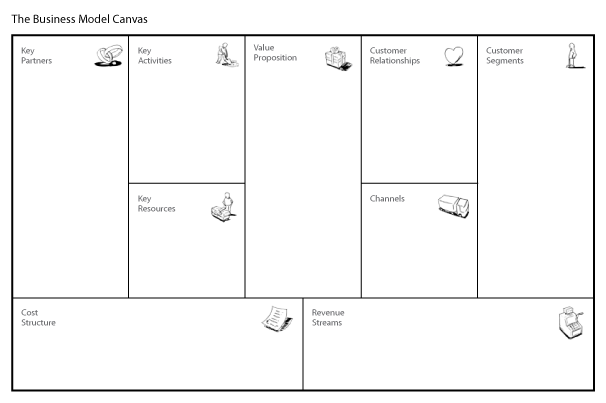
\includegraphics[width=10cm]{business_model_canvas.png}
\end{figure}

\begin{enumerate}
    \item Segmenti di clientela
    \begin{itemize}
        \item Per chi stiamo creando valore?
        \item Chi sono i nostri clienti più importanti?
    \end{itemize}
    \item Proposte di valore
    \begin{itemize}
        \item Quali problemi dei nostri clienti stiamo risolvendo?
        \item Quali bisogni dei nostri clienti stiamo soddisfacendo?
        \item Cosa lega i nostri prodotti e servizi a ciascun segmento di
        clienti?
    \end{itemize}
    \item Canali
    \begin{itemize}
        \item Attraverso quali canali possiamo raggiungere i nostri clienti? 
        \item Quali sono i canali che funzionano meglio? 
        \item Quali sono i canali meno costosi?
    \end{itemize}
    \item Relazioni con i clienti
    \begin{itemize}
        \item Che tipo di relazione ciascun segmento di clienti si aspetta di
        stabilire e mantenere con noi?
        \item Cosa occorre fare per stabilire queste relazioni?
        \item Quanto costa stabilire e mantenere queste relazioni?
    \end{itemize}
    \item Flussi di ricavi
    \begin{itemize}
        \item Cosa sono disposti a pagare i clienti? 
        \item Come preferirebbero pagare i clienti? 
        \item Quanto ciascun flusso di ricavi contribuisce ai ricavi totali?
    \end{itemize}
    \item Risorse chiave
    \begin{itemize}
        \item Quali risorse occorre possedere per poter creare valore? 
        \item Quali altre risorse sono necessarie?
    \end{itemize}
    \item Attività chiave
    \begin{itemize}
        \item Quali attività è indispensabile svolgere per creare valore?
    \end{itemize}
    \item Partner chiave
    \begin{itemize}
        \item Chi sono i nostri partner più importanti?
        \item Chi sono i fornitori più importanti?
        \item Quali risorse forniscono i nostri partner? 
        \item Quali attività svolgono i nostri partner?
    \end{itemize}
    \item Struttura di costo
    \begin{itemize}
        \item Quali sono i principali costi del modello
        di business?
        \item Quali risorse chiave sono più costose?
        \item Quali attività chiave sono più costose?
    \end{itemize}
\end{enumerate}

\subsection{Business Plan}

Il \gls{bizplan} contiene informazioni su:
\begin{itemize}
    \item Il \emph{prodotto o il servizio} che si intende offrire
    \item Il \emph{mercato} in cui l’impresa andrà ad operare
    \item La \emph{strategia} e l’implementazione della stessa
    \item Il \emph{gruppo dirigente}
    \item Le \emph{previsioni finanziarie}
\end{itemize}

\subsection{Fonti di finanziamento}

In linea di principio non serve un capitale proprio, tuttavia l’imprenditore
potrebbe raccogliere capitale da soci esterni (capitale di rischio) e/o credito
(capitale di debito) sulla base della sua idea di business.

La presenza di capitale proprio dei fondatori garantisce i creditori
da rischio di insolvenza e segnala credibilmente il valore dell’idea di
business a finanziatori esterni.

Per sostenere la crescita è necessario raccogliere capitale da finanziatori
esterni specializzati:
\begin{itemize}
    \item Banche
    \item Venture Capitalists
    \item Business Angels
    \item Crowdfunding
    \item Sussidi pubblici
\end{itemize}

\section{Morte di un'impresa}
L’impresa ha durata indefinita, infatti non muore con l’imprenditore, ma
rischia però di ``morire'' se non realizza profitti e dunque non riesce a
remunerare i fattori produttivi.

\subsection{Tipologie}

\begin{itemize}
    \item \emph{Fallimento (scioglimento coatto)}: l’impresa è sciolta per
    ordine del tribunale, i suoi beni vengono venduti
    \item \emph{Liquidazione (scioglimento volontario)}: vendita volontaria dei beni decisa dai
    soci. La ``morte'' per liquidazione non sempre ha un’accezione negativa.
    \item \emph{Acquisizione/Fusione}: l’impresa viene assorbita da un'altra
    impresa. La ``morte'' per fusione ha spesso un'accezione positiva.
\end{itemize}

\section{Tipologie di imprese}
\begin{enumerate}
    \item Proprietà
    \begin{itemize}
        \item \emph{Proprietà pubblica}: il proprietario è un ente pubblico
        (es: lo Stato)
        \item \emph{Proprietà privata}
    \end{itemize}
    \item Obiettivo
    \begin{itemize}
        \item \emph{Profit}: l’obiettivo principale è il profitto
        \item \emph{No profit}: l’obiettivo è uno scopo alternativo, spesso
        socialmente rilevante
    \end{itemize}
    \item Dimensione
    \begin{itemize}
        \item \emph{Grandi imprese}: addetti $\ge 250$ e fatturato $> 50$ \textsc{mil} \euro
        \item \emph{Medie imprese}: addetti $50-249$ e fatturato $10-50$ \textsc{mil} \euro
        \item \emph{Piccole imprese}: addetti $< 50$ e fatturato $< 10$ \textsc{mil} \euro
        \item \emph{Microimprese}: addetti $< 10$ e fatturato $\le 2$ \textsc{mil} \euro
    \end{itemize}
    \item Tipologia di output
    \begin{itemize}
        \item \emph{Beni materiali}
        \begin{itemize}
            \item Imprese agricole: producono beni con processi naturali legati 
            alla terra
            \item Imprese industriali/manifatturiere: compiono trasformazioni
            tecniche dei beni
        \end{itemize}
        \item \emph{Servizi}
        \begin{itemize}
            \item Imprese di trasporto e telecomunicazioni
            \item Distribuzione di energia elettrica, gas, acqua
            \item Negozi
            \item Banche
            \item Assicurazioni
        \end{itemize}
    \end{itemize}
    \item Numero di output
    \begin{itemize}
        \item \emph{Monoprodotto}: imprese che producono/vendono un solo prodotto
        \item \emph{Diversificate}: imprese che producono/vendono vari prodotti/servizi
        da qualche punto di vista imparentati tra loro
        \item \emph{Conglomerali}: imprese che producono/vendono vari prodotti/servizi
        poco imparentati tra loro. Spesso esiste un core business
        (prodotto/servizio ritenuto più importante)
    \end{itemize}
    \item Consumatore
    \begin{itemize}
        \item \emph{Wholesale (all’ingrosso)}: imprese che producono e vendono prodotti
        intermedi ad altre imprese che, a loro volta, li utilizzano nel loro processo
        produttivo
        \item \emph{Retail (al dettaglio)}: imprese che vendono il prodotto al consumatore in
        un mercato finale
    \end{itemize}
    \item Localizzazione delle attività produttive
    \begin{itemize}
        \item \emph{Multinazionali}: hanno interessi economici e attività produttive in più di
        una nazione
        \item \emph{Nazionali}
    \end{itemize}
\end{enumerate}

\section{Forme giuridiche}

\subsection{Imprese individuali}
Sono costituite da un'\emph{unica persona fisica}.

Il titolare (\gls{piccoloimpr}) ha \gls{respill} delle obbligazioni dell'impresa con tutto il patrimonio personale.

È tipica di attività come: commercialista, architetto, ingegnere, medico,
consulente di vario genere\dots

\subsubsection{Impresa familiare}
È un'estensione dell’impresa individuale, quando l’imprenditore
si avvale in modo continuativo della prestazione lavorativa dei familiari
(parentela fino al $3^o$ grado e affinità fino al $2^o$ grado).

\proandcons{
    Semplicità nella costituzione e lo scioglimento dell'impresa.
    Non è richiesto il versamento del capitale

    Pochi obblighi contabili
    
    Autonomia e velocità decisionale
}{
    \Gls{respill}

    In caso di forti guadagni le imposte crescono a causa delle aliquote
    progressive previste dall'Irpef
}


\subsection{Imprese collettive}

\subsubsection{Società di persone}

\paragraph{Società semplice (s.s.)} Riservata ad \emph{attività economiche non commerciali}
(attività agricole e per la gestione di patrimoni immobiliari).

\paragraph{Società in nome collettivo (s.n.c.)} Può esercitare sia attività di
impresa commerciale, sia attività economiche non commerciali.

\paragraph{Società in accomandita semplice (s.a.s.)} Si distingue tra:
\begin{itemize}
    \item Soci accomandatari: si assumono in forma illimitata e solidale le
    responsabilità connesse all'esercizio dell'impresa
    \item Soci accomandanti: affidano in gestione i loro capitali ad altri soci e
    sono responsabili solo del capitale conferito
\end{itemize}

\proandcons{
    Costituzione e tenuta della contabilità relativamente semplici
    
    Procedure burocratiche, fiscali, contabili e tributarie minime
    
    Non è obbligatorio il versamento di un capitale minimo da parte dei
    soci (l’importo è stabilito dal contratto sociale)
}{
    Responsabilità illimitata (a parte accomandanti della s.a.s.) e solidale.
    Se un socio non adempie, il debito dovrà essere saldato dagli altri.

    Minore autonomia decisionale, problemi di coordinamento 
}

\subsubsection{Società di capitali}

\paragraph{Società a responsabilità limitata (s.r.l.)}
\begin{itemize}
    \item Capitale sociale (ossia la proprietà) è diviso in quote
    \item Nell’assemblea dei soci si vota per la quota posseduta
    \item Capitale minimo: 10.000 \euro
\end{itemize}

\paragraph{Società a responsabilità limitata semplificata (S.r.l.s.)}
\begin{itemize}
    \item Forma di s.r.l. recentemente introdotta (2012) dalla legislazione per
    favorire l’imprenditorialità
    \item Capitale minimo: 1 \euro
    \item Capitale massimo: 9.999,99 \euro
    \item Modello standard dell’atto di costituzione della società, per la stipula
    dell'atto costitutivo non sono dovuti onorari notarili
\end{itemize}

\paragraph{Società per azioni (s.p.a.)}
\begin{itemize}
    \item Il patrimonio sociale è costituito da azioni
    \item Le azioni sono quote di partecipazione liberamente trasferibili
    \item Possibile quotazione in Borsa
    \item Capitale minimo: 50.000 \euro
\end{itemize}

\paragraph{Società in accomandita per azioni (s.a.p.a.)}
\begin{itemize}
    \item I soci si distinguono in accomandatari e accomandanti
\end{itemize}

\proandcons{
    Responsabilità limitata
    
    Gestione può essere affidata anche ai non soci
    
    Tassazione sulle imprese
    
    Utili possono essere distribuiti ai soci nei momenti fiscalmente più
    convenienti
    
}{
    Adempimenti burocratici e fiscali sono numerosi e complessi (es.
    contabilità ordinaria)
    
    Obbligatorio il conferimento di capitale iniziale

    Maggiori obblighi di trasparenza e di governance
}

\subsubsection{Società cooperative}

\begin{itemize}
    \item Imprese che pur svolgendo un’attività economica non hanno l’obiettivo di
    distribuire utili significativi in capo ai soci
    \item Devono reinvestire i profitti nell’attività imprenditoriale
    \item Qualora dette imprese non dovessero rispettare questi requisiti perderebbero
    il diritto alle importanti agevolazioni fiscali di cui possono beneficiare
    \item Si distinguono in società cooperative a \gls{respill} e) società
    cooperative a \gls{resplim}
\end{itemize}

\subsubsection{Startup innovative}
Dal 2012, esiste una nuova tipologia d'impresa, le \emph{startup innovative}.

\paragraph{Requisiti}

\begin{itemize}
    \item  Essere attive da meno di 5 anni
    \item Avere sede principale in Italia, o in altro Paese membro dell’Unione Europea, purché ci sia una
    sede produttiva o una filiale in Italia
    \item Avere un fatturato annuo inferiore a 5 milioni di euro
    \item Non distribuire utili
    \item Non essere costituite da fusione, scissione societaria o a seguito di cessione di azienda o di ramo
    di azienda
    \item Sviluppare, produrre e commercializzare prodotti o servizi innovativi ad \emph{alto valore tecnologico},
    ed essere in possesso di almeno uno dei tre seguenti criteri:
    \begin{itemize}
        \item Almeno il 15\% del maggiore tra fatturato e costi annui è ascrivibile ad attività di ricerca e
        sviluppo
        \item La forza lavoro complessiva è costituita per almeno 1/3 da dottorandi, dottori di ricerca o
        ricercatori, oppure per almeno 2/3 da soci con laurea magistrale
        \item L’impresa è titolare, depositaria o licenziataria di un brevetto registrato
    \end{itemize}
\end{itemize}

\paragraph{Agevolazioni}

\begin{itemize}
    \item Agevolazioni per startup innovative:
    \item Esonero pagamento dei diritti camerali annuali e imposte di bollo
    \item Gestione societaria flessibile: l’atto costitutivo delle startup innovative costituite in
    una SRL può prevedere categorie di quote che non attribuiscono diritti di voto o che ne
    attribuiscono in misura non proporzionale alla partecipazione
    \item Regime speciale per le perdite: 2 anni (al posto di 1) di tempo per il ripianamento
    delle perdite superiori ad un terzo del capitale
    \item Assunzioni del personale: contratti a tempo determinato dalla durata minima di 6
    mesi a massimo 36 mesi con rinnovo, stipendi flessibili, ecc..
    \item Incentivi fiscali per le persone fisiche e giuridiche che investono nella startup
    \item Equity crowdfunding
    \item Accesso facilitato e gratuito al credito del Fondo di Garanzia per le Piccole e Medie
    Imprese (garanzia del Governo fino a coprirne l'80% del credito erogato dalla banca)
    \item Esonero dalla procedura di fallimento aziendale e possibilità per l'imprenditore di
    intraprendere un nuovo progetto in tempi brevi
\end{itemize}

\chapter{Contabilità Esterna}
La \gls{contabilita} si occupa di gestire le informazioni pubbliche redatte da 
imprese e altri soggetti (per esempio gli enti pubblici), secondo criteri omogenei 
stabiliti dalla legge per ragioni di efficacia e trasparenza.

Le informazioni devono quindi essere:
\begin{itemize}
    \item \emph{accertate}: documentate secondo rigide regole formali
    \item \emph{sintetiche}: si riportano entrate/uscite
    \item \emph{storiche}: relative a eventi avvenuti in un dato periodo di tempo
\end{itemize}

I destinatari della contabilità esterna sono gli \glspl{shareholder} e gli
\glspl{stakeholder}, che studiano la contabilità per stabilire:
\begin{itemize}
    \item La capacità dell’impresa di creare valore economico
    \item Le determinanti della redditività
    \item La sostenibilità finanziaria del modello di business
    \item La capacità dell’impresa di far fronte alle obbligazioni assunte
    \item La redditività conseguita a fronte della redditività attesa
\end{itemize}
 
\section{Bilancio di esercizio}
È un documento redatto con la finalità di informare i diversi \glspl{stakeholder}
sulla situazione economica, finanziaria e patrimoniale dell’impresa in un determinato
\gls{esercizio}.

Il bilancio è \emph{pubblico}, \emph{obbligatorio}, che sintetizza le operazioni
di gestione condotte dall’impresa nel corso di un esercizio contabile (anno solare),
soggetto a \emph{regolamentazione}.

Il bilancio deve comunicare se e quanto l’impresa è:
\begin{itemize}
    \item In \emph{equilibrio reddituale}
    \begin{itemize}
        \item La gestione dell’impresa da parte del management è stata in grado di generare un reddito ``sufficiente''?
        \item Ciò che resta dei ricavi delle vendite e degli altri proventi dopo avere sostenuto i costi
        (dipendenti, fornitori, creditori, fisco...) è all’altezza delle aspettative di remunerazione dei proprietari?
    \end{itemize}
    \item In \emph{equilibrio finanziario}
    \begin{itemize}
        \item Le entrate dell’impresa permettono di far fronte nei tempi richiesti agli obblighi sottoscritti nei confronti di terzi?
    \end{itemize}
\end{itemize}

\subsection{Esempio di bilancio}
\textit{Vendo prodotti per 100 al tempo $T$ (il prodotto è scambiato al tempo $T$), incasso il pagamento per 100 dal cliente al tempo $T+1$.}
\begin{enumerate}
    \item Logica reddituale: \quad
    $
        \textbf{Utile}
        \begin{cases}
            \text{Ricavi}_T = +100\\
            \text{Ricavi}_{T+1} = 0
        \end{cases}
    $
    \item Logica finanziaria: \quad
    $
    \textbf{Disponibilità Liquide}
    \begin{cases}
        \text{Cassa}_T = 0\\
        \text{Cassa}_{T+1} = +100
    \end{cases}
    $
\end{enumerate}

\subsection{Principi contabili}
Sono criteri che stabiliscono:
\begin{itemize}
    \item i fatti da registrare
    \item le modalità attraverso le quali contabilizzare le operazioni di gestione
    \item i criteri di valutazione e di esposizione dei valori di bilancio
\end{itemize}

Le informazioni devono essere \emph{complete}, \emph{veritiere}, \emph{comparabili tra imprese}

\subsection{Normativa}
Un \gls{bilancio} redatto in accordo ai principi \gls{ifrsias} (International Financial
Reporting Standards/International Accounting Standards).

I principi \gls{ifrsias} sono obbligatori per le società quotate.

\subsection{Documenti}

\begin{itemize}
    \item \textbf{\Gls{sp} (SP):} descrive la situazione patrimoniale dell’impresa in un determinato istante
    \item \textbf{\Gls{ce} (CE):} riassume i flussi di ricavi e costi avvenuti nell’esercizio
    \item \textbf{\Gls{rf}:} presenta i flussi di cassa che hanno interessato l’impresa nell’esercizio
    \item \textbf{Nota integrativa:} contiene le regole, le ipotesi e le convenzioni utilizzate dall’impresa per redigere Stato Patrimoniale e Conto Economico
\end{itemize}

Nella normativa italiana, le aziende devono anche redigere:
\begin{itemize}
    \item \textbf{Relazione degli amministratori}: riporta le considerazioni del management in merito all’andamento dell’impresa
    \item \textbf{Relazione dei sindaci}, o comunque dell’organo preposto al controllo di legalità
    \item \textbf{Relazione della società di revisione}: attesta l’oggettiva correttezza del bilancio, la rispondenza ai principi contabili utilizzati per la redazione del bilancio, la veridicità delle informazioni in esso contenute
\end{itemize}

\subsection{Limiti}
A causa della sua valenza esterna e dei tempi necessari alla sua  predisposizione,
\emph{il bilancio manca di analiticità e tempestività}.

Le informazioni riportate nel bilancio sono sintetiche e aggregate, e risultano
disponibili anche dopo settimane o  addirittura mesi dalla chiusura dello stesso.
\emph{Tempi di approvazione ordinari sono entro 120 giorni dalla chiusura dell’esercizio}.

Perciò tali informazioni non costituiscono un supporto adeguato per le singole decisioni del management,
per le quali è necessario disporre di \emph{indicazioni più puntuali e tempestive}, di cui si occupa la
\emph{contabilità interna}.

\section{Stato Patrimoniale}
È l'insieme delle \emph{risorse} a disposizione dell’impresa per produrre e vendere, dette \gls{attivita},
e dei \emph{diritti} vantati sull’impresa da parte dei finanziatori, detti \gls{passivita}.

La grandezza utilizzata per rappresentare sia le risorse sia i diritti è il \emph{valore monetario}.

Solitamente non compaiono nelle attività le risorse umane, perchè su tali risorse
nessuno dei soggetti che hanno conferito capitale può vantare diritti di controllo.

\subsection{Identità fondamentale}
\begin{equation*}
    \text{Totale Attività} \equiv \text{Totale Passività} + \text{Patrimonio Netto}
\end{equation*}

\subsubsection{Esempio}
\begin{tabular}{| l r | l r |}
    \hline
    \textbf{Attività} & & \textbf{Patrimonio netto e passività} & \\
    \hline
    Macchinario & 300 & Capitale sociale & 150 \\
    Cassa       & 50  & Debito           & 200 \\ 
    \hline 
\end{tabular}
\newline
\newline
$\text{Totale Attività} = \text{Totale Passività} + \text{Patrimonio Netto} = 300 + 50 = 150 + 200 = 350$

\subsection{Attività}

\subsubsection{Attività non correnti}
Sono risorse utilizzate anche oltre l’esercizio contabile, con utilità pluriennale. Si distinguono tra:
\begin{itemize}
    \item \emph{a vita definita}: hanno un effetto nel tempo limitato e stimabile
    \item \emph{a vita non definita}: non vi è un limite prevedibile al periodo
    durante il quale ci si attende che l’attività generi benefici economici
\end{itemize}

\paragraph{Immobilizzazioni materiali} risorse aventi natura prevalentemente ``fisica''
ed il cui impiego naturale per l’impresa si estende oltre l’esercizio di riferimento:
\begin{itemize}
    \item Immobili, impianti e macchinari di proprietà
    \item Beni in locazione (es. flotta auto aziendale)
    \item Investimenti immobiliari
\end{itemize}

\subparagraph{Iscrizione a bilancio} al costo d'acquisto.
\subparagraph{Valorizzazione negli anni successivi} dipende dall’attività (vita utile).

\paragraph{Immobilizzazioni immateriali} attività prive di consistenza fisica, controllate
dall’impresa e in grado di produrre benefici economici:
\begin{itemize}
    \item Costi di sviluppo
    \item Brevetti e licenze
    \item Avviamento: eccedenza del costo di un’acquisizione aziendale rispetto
    al valore contabile delle attività e delle passività dell’impresa acquisita
\end{itemize}

\subparagraph{Iscrizione a bilancio}
\begin{itemize}
    \item Attività acquisita all’esterno: costo di acquisto più costi direttamente imputabili
    \item Attività autoprodotta: costi direttamente imputabili alla fase di sviluppo
\end{itemize}

\subparagraph{Valorizzazione negli anni successivi} dipende dall’attività (vita utile)

\paragraph{Immobilizzazioni finanziarie}
\begin{itemize}
    \item Partecipazioni: azioni e quote societarie di altre imprese
    \item Titoli, crediti finanziari, altre attività finanziarie
\end{itemize}

\subparagraph{Iscrizione a bilancio} al costo d'acquisto
\subparagraph{Valorizzazione negli anni successivi} tipicamente \gls{fairvalue}:
rivalutazioni/svalutazioni

\subsubsection{Valorizzazione}

\begin{itemize}
    \item Nel caso di \emph{attività a vita utile definita} si usa il metodo dell'ammortamento.
    \item Nel caso di \emph{attività a vita utile non definita} è necessaria la stima del \gls{fairvalue}.
\end{itemize}


\paragraph{Ammortamento} valore della ``quota'' della risorsa che viene ``consumata''
dalla produzione o “deperisce” per obsolescenza tecnologica
\begin{itemize}
    \item a quote costanti: in parti uguali lungo la vita utile del bene
    \item a quote decrescenti: maggiore ``consumo'' del bene nei primi anni
    \item secondo le quantità prodotte: ``consumo'' del bene basato sull’utilizzo
    effettivo o sulla produzione ottenuta dal bene
\end{itemize}

\subparagraph{Calcolo dell'ammortamento a quote costanti} dove $V_0$ è il costo
di acquisto della risorsa, $V_f$ valore presunto di cessione dopo $T$ anni.

\begin{equation*}
    \text{Ammortamento} = \frac{V_0 - V_f}{T}
\end{equation*}

\subparagraph{Valore della risorsa in ciascun anno $T$}
\begin{equation*}
    V(t) = V(t-1) - \text{Ammortamento}
\end{equation*}

\subparagraph{Valorizzazione negli anni successivi} per le attività materiali è pari al
costo di acquisto al netto degli ammortamenti cumulati fino all’anno corrente

\subparagraph{\Gls{imptest}} valutazione periodica/\emph{una tantum} quando la
risorsa mostra una perdita di valore giudicata durevole

\paragraph{Fair value} corrispettivo al quale un'attività può essere scambiata,
o una passività estinta, tra parti consapevoli e disponibili, in una transazione
tra parti terze e indipendenti.

È una valutazione annua.

\subparagraph{Calcolo del \gls{fairvalue}}
$\text{FV}(T)$: prezzo che un potenziale acquirente è disposto a pagare all'anno $T$.
\begin{itemize}
    \item Se $\text{FV}(T) > V(T-1) \Rightarrow$ rivalutazione
    \item Se $\text{FV}(T) < V(T-1) \Rightarrow$ svalutazione
\end{itemize}

\subparagraph{\Gls{imptest}} obbligatorio annualmente per attività a vitanon definita e avviamento

\subsubsection{Attività correnti}
Attività liquide o destinate a trasformarsi in liquidità entro l’esercizio successivo.

\paragraph{Rimanenze di magazzino} beni posseduti per la vendita o impiegati nei
processi produttivi o nella prestazione di servizi
\begin{itemize}
    \item Materie prime
    \item Semilavorati
    \item Prodotti finiti
\end{itemize}

\subparagraph{Iscrizione a bilancio} valore minore tra \gls{costo} e \gls{valrealizzo}

\paragraph{Crediti commerciali} crediti verso clienti a cui si è accordata una dilazione di pagamento.
\subparagraph{Iscrizione a bilancio} presumibile \gls{valrealizzo} (al netto del corrispondente fondo rischi)

\paragraph{Lavori in corso su ordinazione} contratti stipulati specificamente per la costruzione di un bene o di una combinazione di beni.
\subparagraph{Iscrizione a bilancio} valore pattuito nella commessa in proporzione allo stato di avanzamento

\paragraph{Disponibilità liquide (Cassa)} valori contanti in cassa aziendale,
depositi bancari e postali, titoli di stato di breve (e quindi facilmente liquidabili).
\subparagraph{Iscrizione a bilancio} \gls{valrealizzo} (ammontare del denaro)

\paragraph{Attività finanziarie correnti}
\begin{itemize}
    \item Titoli
    \item Crediti finanziari 
    diverse dalle partecipazioni, detenute per negoziazione o disponibili per la vendita
    \item Altre partecipazioni
    \item Derivati di copertura relativi ad attività correnti
    \item Altre voci residuali
\end{itemize}
\subparagraph{Iscrizione a bilancio} \gls{fairvalue}

\paragraph{Ratei e risconti attivi} sono voci di aggiustamento delle entrate e
delle uscite di cassa rispetto ai costi e ai ricavi di competenza dell’esercizio.

\subparagraph{Ratei attivi} (\emph{ricavo posticipato}) ricavi la cui competenza economica è già maturata al 
termine dell’esercizio, mentre il corrispondente flusso monetario non è ancora avvenuto.
\subparagraph{Risconti attivi} (\emph{costo anticipato}) costi già sostenuti dall’impresa la cui competenza
economica è relativa ad esercizi futuri.
\subparagraph{Iscrizione a bilancio}: gli IAS non trattano specificamente dei
ratei e dei risconti considerandoli all'interno di altre classi di debiti e crediti

\subsection{Patrimonio netto e Passività}

\subsubsection{Patrimonio netto}
Il \gls{patrnetto} comprende:

\paragraph{Capitale emesso} capitale conferito dagli azionisti all’impresa all’atto della sottoscrizione
\begin{itemize}
    \item del capitale iniziale
    \item i aumenti di capitale (gratuiti, a pagamento con sovrapprezzo e senza sovrapprezzo)
\end{itemize}
\subparagraph{Iscrizione a bilancio} somma del valore delle singole quote

\paragraph{Riserva sovrapprezzo azioni} capitale ``aggiuntivo'' conferito dagli
azionisti all’atto della sottoscrizione di aumenti di capitale a pagamento.
\subparagraph{Iscrizione a bilancio} 
\begin{equation*}
    \text{(Valore acquisto azioni)} - \text{(Valore nominale azioni)}
    \times \text{(Numero di azioni dell'aumento capitale)}
\end{equation*}

\paragraph{Riserva da rivalutazione} incorpora gli effetti delle modifiche di
valore derivanti dall’applicazione del criterio del \gls{fairvalue}.
\subparagraph{Iscrizione a bilancio}
\begin{equation*}
    \text{(Fair value dell'attivo)} - \text{(Valore precendente dell'attivo)}
\end{equation*}

\paragraph{Utile (perdita) portato a nuovo} somma di tutti gli \glspl{utile} che
l’impresa ha deciso di non distribuire agli azionisti, ad esempio, per motivi di
autofinanziamento interno.

\paragraph{Utile (perdita) di esercizio} risultato economico di pertinenza degli
azionisti maturato nell’esercizio cui si riferisce il bilancio.
È pari al valore riportato alla fine del Conto Economico.


\textbox{Gli \glspl{utile} sono le uniche voci dello Stato Patrimoniale che 
possono assumere valori negativi.}

\subsubsection{Passività finanziarie}
Diritti vantati da soggetti terzi (\emph{non azionisti}) che hanno finanziato l’impresa.
\begin{itemize}
    \item Passività \emph{non correnti}: non esauriscono il loro impatto all’interno dell’\gls{esercizio} successivo
    \item Passività \emph{correnti}: esauriscono il loro impatto all’interno dell’\gls{esercizio} successivo 
\end{itemize}
Di solito prevedono il pagamento di un interesse.

\paragraph{Obbligazioni} sono titoli di credito emessi per la raccolta di capitale di debito.

L’obbligazione è costituita da un certificato che rappresenta una frazione, di uguale
valore nominale e con uguali diritti, di un’operazione di finanziamento.

La società emittente garantisce ai sottoscrittori la riscossione di un interesse
ed il rimborso del capitale a scadenza, o sulla base di un piano di ammortamento predefinito.

\subparagraph{Iscrizione a bilancio} \gls{fairvalue}, cioè il valore da riconoscere
a chi oggi si assume il titolo debito

\paragraph{Debiti verso banche}
\subparagraph{Iscrizione a bilancio} \gls{fairvalue}

\paragraph{Fondo TFR e altri fondi relativi al personale} obblighi verso i dipendenti
da liquidare all’interruzione del rapporto lavorativo (\gls{TFR}) o alla data della pensione
(fondo pensione). I fondi sono creati con \emph{accantonamenti annui al TFR nel Conto Economico}.
\subparagraph{Iscrizione a bilancio} stima attuariale di ente indipendente

\paragraph{Fondo rischi e oneri} costi e oneri di esistenza certa o probabile che
alla data di chiusura dell’esercizio sono indeterminati nell’ammontare o nella data
di sopravvenienza (per esempio, un fondo  garanzia prodotti, contenziosi fiscali\dots oppure
fondi creati con accantonamenti annui).
\subparagraph{Iscrizione a bilancio} \gls{fairvalue}

\paragraph{Debiti commerciali} pagamenti differiti verso i fornitori sorti per costi
relativi all’acquisto di materie prime, servizi, costi per godimento di beni di terzi.
In genere sono passività correnti.
\subparagraph{Iscrizione a bilancio} costo d'acquisto

\paragraph{Debiti per imposte} imposte sul reddito dell’esercizio calcolate sulla
base della stima del reddito imponibile.
\subparagraph{Iscrizione a bilancio} valore che si prevede di pagare alle autorità
fiscali applicando le aliquote e la normativa fiscale vigenti (o approvate alla
data di chiusura dell’esercizio)

\paragraph{Ratei e risconti passivi} i ratei e i risconti sono voci di aggiustamento
delle entrate e delle uscite di cassa rispetto ai costi e ai ricavi di competenza dell’esercizio.
\subparagraph{Rateo passivo} (\emph{costo posticipato})
\subparagraph{Risconto passivo} (\emph{ricavo anticipato})
\subparagraph{Iscrizione a bilancio} gli IAS non trattano specificatamente dei ratei
e dei risconticonsiderandoli all'interno di altre classi di debiti e crediti

\section{Conto Economico}
Documento di bilancio che presenta i \emph{flussi economici in entrata ed uscita} dall’impresa nel corso
dell’esercizio contabile, determina l’\emph{utile di esercizio} dell’impresa come differenza tra i costi e i
ricavi dell’esercizio e mostra se e quanto l’impresa \emph{remunera il capitale investito}.

\subsection{Principio di competenza economica}
Stabilisce che solo i costi e i ricavi di competenza di un esercizio contribuiscono
a formare l’utile di esercizio. 

\paragraph{Ricavi di competenza}
valore dei beni alienati e/o dei servizi erogati nel
corso dell’esercizio.

I ricavi vengono registrati nel \gls{contoeconomico} nell’anno in cui è avvenuta l’alienazione
del bene/erogazione del servizi anche se l’entrata di cassa (incasso) è
precedente o successiva.

Applicando il principio di competenza economica, possono verificarsi le
seguenti situazioni per quanto riguarda i \emph{ricavi}:
\begin{itemize}
    \item Il prodotto/servizio è stato consegnato e la controparte ha pagato
    \begin{itemize}
        \item Un Ricavo è registrato nel CE dell’esercizio
        \item Contestualmente, aumentano le Attività nello SP\footnote{\gls{sp}} (Cassa)
    \end{itemize}
    \item Il prodotto/servizio è stato consegnato, ma la controparte non ha pagato
    \begin{itemize}
        \item Un Ricavo è registrato nel CE dell’esercizio
        \item Contestualmente, aumentano le Attività nello SP (Credito Commerciale)
    \end{itemize}
\end{itemize}

\paragraph{Costi di competenza}
valore delle risorse utilizzate per ``produrre'' i ricavi.

I costi vengono registrati nel CE nell’anno in cui contribuiscono alla
produzione anche se l’uscita di cassa (esborso) è precedente o
successiva.

Applicando il principio di competenza economica, possono verificarsi le
seguenti situazioni per quanto riguarda i costi:
\begin{itemize}
    \item L’impresa ha usufruito di un bene/servizio e ha pagato la controparte
    \begin{itemize}
        \item Un Costo è registrato nel CE dell’esercizio
        \item Contestualmente, dimuniscono le Attività nello SP (Cassa)
    \end{itemize}
    \item L’impresa ha usufruito di un bene/servizio, ma non lo ha ancora pagato
    \begin{itemize}
        \item Un Costo è registrato nel CE dell’esercizio
        \item Contestualmente, aumentano le Passività nello SP (Debito Commerciale)
    \end{itemize}
\end{itemize}

\subsection{Presentazione del conto economico}

\paragraph{Per natura}
i costi sono aggregati secondo la loro natura (es: acquisti di
materiali, costi del personale)

\paragraph{Per destinazione (o del ``costo del venduto'')}
i costi sono aggregati secondo la loro funzione all’interno dell’impresa (parte del costo di
realizzazione dei beni venduti, costi di distribuzione, costi amministrativi)

\subsection{Gestioni}
Il \gls{contoeconomico} è un conto scalare in cui ricavi/proventi e costi/oneri sono distinti per ``gestioni'',
delle quali si può identificare il reddito generato.

\subsubsection{Gestione Operativa}

\paragraph{Ricavi operativi}
\begin{itemize}
    \item Ricavi derivanti dalla vendita di beni/erogazione di servizi
    \item Ricavi dell’attività tipica e ordinaria dell’impresa
\end{itemize}

\paragraph{Altri proventi operativi}
\begin{itemize}
    \item Ricavi derivanti dall’utilizzo da parte di terzi di beni dell’impresa (ad
    esempio: canoni di affitto, royalties)
\end{itemize}

\paragraph{Acquisti di materie primi}
\begin{itemize}
    \item Costo delle materie prime acquistate e dei materiali
    di consumo
\end{itemize}

\paragraph{Costi del personale}
\begin{itemize}
    \item Salari e stipendi
    \item Oneri sociali e riferiti al trattamento di
    fine rapporto e più in generale ai piani di benefici per i dipendenti
\end{itemize}

\paragraph{Altri costi operativi}
\begin{itemize}
    \item Costi dell’energia
    \item Costi di manutenzione e riparazione ordinarie
    \item Costi di distribuzione, commerciali e amministrativi
    \item Canoni di affitti e i canoni di leasing operativi
\end{itemize}

\paragraph{Costi per lavori interni capitalizzati}
\begin{itemize}
    \item Costi per migliorie, ammodernamento
    e trasformazione delle attività materiali
\end{itemize}

\paragraph{Variazione delle rimanenze}
Si indica la \emph{differenza algebrica tra il valore delle rimanenze finali e quelle
iniziali}, eliminando così l’effetto di distorsione dei costi di produzione che non sono di
competenza economica.

\begin{itemize}
    \item Materie prime
    \item Prodotti finiti
    \item Work in progress (prodotti in corso di lavorazione)
    \item Semilavorati
\end{itemize}

\paragraph{Ammortamento}
\begin{itemize}
    \item Costo \emph{non cash}
    \item Nel CE si inserisce la \emph{quota} della risorsa in questione consumata nell'\gls{esercizio}.
    \item Corrisponde ad una riduzione tra le attività dello SP
\end{itemize}

Per esempio, se l'ammortamento è a quote costanti per una vita utile
di 10 anni, la quota sarà un decimo del costo d'acquisto.

\paragraph{Accantonamento}
\begin{itemize}
    \item Costo \emph{non cash}, creato per far fronte a impegni incerti per il loro ammontare e/o per la
    loro scadenza.
    \item Nel CE è incluso nel costo del personale dell’esercizio
    \item Corrisponde ad un aumento delle passività dello SP
\end{itemize}

\paragraph{Plusvalenze/minusvalenze da realizzo di attività non correnti}
\begin{itemize}
    \item Differenza tra il ricavo ottenuto a seguito della cessione di un’attività non corrente ed il
    valore iscritto a bilancio.
\end{itemize}

\paragraph{Ripristini o rivalutazioni/svalutazioni di valore di attività non correnti}
\begin{itemize}
    \item Voce che include gli effetti dell’applicazione del criterio del \gls{fairvalue} sulle
    attività non correnti.
    \item Quando il valore contabile di una attività materiale o immateriale aumenta
    per effetto di una \emph{rivalutazione}, l’incremento viene attribuito
    direttamente alla riserva di rivalutazione nel PN.
    \item Un incremento deve essere \emph{rilevato a CE} solo se rappresenta il
    \emph{recupero di valore di una svalutazione precedente} imputata al
    CE e relativa allo stesso bene.
    \item L’effetto di una \emph{svalutazione} deve invece essere imputato \emph{direttamente
    a CE}, a meno che non sia successiva ad una precedente rivalutazione
    dello stesso bene contabilizzata a PN (in quel caso si riduce la riserva
    fino ad estinguerla, l’eventuale eccedenza si imputa a CE) 
\end{itemize}

\subsubsection{Gestione Finanziaria}

\paragraph{Proventi finanziari}
\begin{itemize}
    \item Interessi attivi su disponibilità liquide
    \item Proventi da partecipazioni
    \item Altri proventi finanziari derivanti da titoli iscritti nell’attivo (interessi
    attivi su prestiti, obbligazioni, dividendi su azioni)
    \item Variazioni positive fair value di attività finanziarie
\end{itemize}

\paragraph{Oneri finanziari}
\begin{itemize}
    \item Interessi e gli altri oneri sostenuti in relazione all’ottenimento di
    finanziamenti (breve e lungo)
    \item Variazioni negative fair value di passività finanziarie
\end{itemize}

\subsubsection{Gestione Fiscale}
\paragraph{Imposte calcolate sull’esercizio corrente}

\subparagraph{IRES (Imposta sul reddito delle società)}
calcolata sul risultato ante imposte: 24\%

\textbf{Base imponibile}
\begin{itemize}
    \item Risultato prima delle imposte 
    \item Deduzioni ($+$, $-$)
\end{itemize}

\subparagraph{IRAP (Imposta sul reddito delle attività produttive)}
calcolata sul valore aggiunto: 3,9\% (Lombardia, imprese industriali)

\textbf{Base imponibile}
\begin{itemize}
    \item \gls{ebit} 
    \item Costo del personale ($+$)
    \item Svalutazioni ($+$) (crediti, immobilizzazioni..) 
    \item Accantonamenti ($+$)
\end{itemize}

Sono inoltre previste delle deduzioni (es.: costo del personale per
ricercatori, per incremento occupazionale, forfettarie,...) che abbattono la
base imponibile.

\subparagraph{Osservazioni}
\begin{itemize}
    \item Con provvedimenti ad hoc, sono rese possibili riduzioni delle imposte
    per incentivare le imprese a sostenere specifici costi
    \item Esistono anche le imposte indirette (imposte sull’energia, sui trasporti)
\end{itemize}

\subsubsection{Utile del periodo}
Noto anche come \emph{utile netto} o \emph{reddito d'impresa}, è il risultato residuale
delle gestioni.

\begin{itemize}
    \item Si iscrive anche nello SP sotto ``\gls{patrnetto}''
    \begin{itemize}
        \item Utile $> 0 \rightarrow$ aumenta i diritti di competenza degli azionisti
        \item Utile $< 0 \rightarrow$ viene eroso valore per gli azionisti
    \end{itemize}
    \item Nel bilancio consolidato, è obbligatoria l’indicazione del risultato di
    pertinenza di terzi
\end{itemize}

\paragraph{Distribuzione degli utili}
L’Assemblea dei Soci in sede di approvazione del bilancio decide:
\begin{itemize}
    \item Quale quota distribuire ai soci (\emph{dividendi})
    \item Quale quota reinvestire (la quale va ad incrementare il PN come
    \emph{utile portato a nuovo} e resta di competenza degli azionisti, cioè utili che potranno essere
    distribuiti negli esercizi futuri)
\end{itemize}

% Opzionale? C'e' in esame?
% \subsection{Consolidamento}

% \paragraph{Consolidamento partecipazioni (bilancio consolidato)}

% \subparagraph{Controllo congiunto}
% nessuna delle parti controlla singolarmente l’accordo. Le
%     decisioni sulle attività rilevanti richiedono il consenso unanime delle parti che
%     controllano l’accordo collettivamente.
% \subparagraph{Joint-venture societaria}
% controllo congiunto che assume una forma societaria (joint venture corporation)
% in cui i partecipanti (co-ventures) si spartiscono oneri e utili della società
% e sono responsabili esclusivamente per la parte di capitale da loro versato.

% \paragraph{Consolidamento integrale bilanci}
% \begin{enumerate}
%     \item Somma di tutte le voci di attivo/passivo
%     \item Eliminazioni dei flussi tra società controllata e controllante (es. crediti/debiti tra le due
%     società)
%     \item Eliminazione della partecipazione nell’attivo della società controllante
%     \item Rilevazione della parte di PN ed utile di pertinenza di terzi
% \end{enumerate}

% TODO: Controllare?
% \paragraph{Metodo Patrimonio Netto}

\section{Rendiconto Finanziario}

Fornisce informazioni utili agli utilizzatori per rappresentare i 
\emph{flussi finanziari in entrata ed in uscita}
 di un’impresa durante l’esercizio contabile.

\textbox{Il Rendiconto Finanziario non segue il principio di competenza economica.}

\subsection{Flussi Finanziari (cash flows)}
Sono \emph{variazioni di disponibilità liquide}, quali ad
esempio la \emph{cassa}, \emph{investimenti a breve termine altamente liquidi} poiché
convertibili in importi di denaro di ammontare determinato e soggetti a rischi
non significativi di cambiamenti di valore (cash equivalents)

\subsubsection{Schema aggregato del Rendiconto Finanziario}
\begin{tabular}{|l | c |}
    \hline
    Flusso di cassa netto della gestione operativa & A \\
    Flusso di cassa netto per attività di investimento & B \\
    Flusso di cassa netto per attività di finanziamento & C \\
    \hline\grayrow
    Incremento (decremento) delle disponibilità liquide & D=A+B+C \\
    \hline
    Disponibilità liquide all’inizio del periodo & E \\
    \hline\grayrow
    Disponibilità liquide alla fine del periodo & F=D+E \\
    \hline
\end{tabular}

\subsubsection{Flusso di cassa netto della gestione operativa}

\begin{itemize}
\item I flussi finanziari generati dall’attività operativa derivano dallo
\emph{svolgimento dei processi produttivi dell’impresa}.
\item Essi possono essere ricondotti a:
\begin{itemize}
    \item Incassi dalla vendita di prodotti e dalla prestazione di servizi
    \item Incassi da royalties, compensi, commissioni e altri ricavi
    \item Pagamenti a fornitori di materie prime, merci e servizi
    \item Pagamenti a e per conto di lavoratori dipendenti
    \item Proventi finanziari e dividendi ricevuti
    \item Pagamenti per oneri finanziari
    \item Pagamenti o rimborsi di imposte sul reddito
\end{itemize}

\item È un \emph{indicatore chiave} della capacità dell’impresa di generare cassa,
senza dover ricorrere a finanziamenti esterni (\emph{autofinanziamento}), per:
\begin{itemize}
    \item Mantenere efficiente la capacità operativa
    \item Finanziare nuovi investimenti
    \item Rimborsare i prestiti
    \item Pagare dividendi
\end{itemize}

\item E’ strettamente legato al CE e alla variazione di Attività e Passività correnti
nello SP.
\end{itemize}

\subparagraph{Metodo diretto}
esposizione delle principali categorie di incassi e di
pagamenti lordi (incassi dai clienti, pagamenti ai fornitori\dots).

L'uso del metodo diretto è fortemente incoraggiato, perchè consente
una lettura più immediata delle fonti e degli impieghi di liquidità.

Nel metodo diretto, il passaggio da ricavi e costi di competenza economica
alle relative entrate ed uscite finanziarie richiede la
\emph{preventiva ricostruzione dei ricavi e dei costi conseguiti e sostenuti nel periodo}
che vanno poi \emph{rettificati} rispettivamente
\emph{delle parti non riscosse e non pagate nel periodo stesso}.

\vspace{1em}
\begin{tabular}{|l|c|}
    \hline
    Incassi dalla vendita di prodotti e dalla prestazione di servizi & $+$ \\
    \hline
    Incassi da royalties, compensi, commissioni e altri ricavi & $+$ \\
    \hline
    Pagamenti a fornitori di materie prime, merci e servizi & $-$ \\
    \hline
    Pagamenti a e per conto di lavoratori dipendenti & $-$ \\
    \hline
    Proventi finanziari e dividendi ricevuti & $+$ \\
    \hline
    Pagamenti per oneri finanziari & $-$ \\
    \hline
    Pagamenti di imposte sul reddito & $-$ \\
    \hline\grayrow
    Flusso di cassa netto della gestione operativa & $+/-$ \\
    \hline
\end{tabular}

\subparagraph{Metodo indiretto} rettificazione del risultato netto d’esercizio degli effetti
delle operazioni di natura non monetaria (costi non cash), e da variazioni ci
capitale circolante netto.

Si parte sempre dall'utile d'esercizio (prima riga).

\vspace{1em}
\begin{tabular}{|l|c|}
    \hline\grayrow
    Utile del periodo & $-/+$ \\
    \hline
    Ammortamenti & $+$ \\
    \hline
    Accantonamenti & $+$ \\
    \hline
    Plusvalenze (minusvalenze) da realizzo di attività non correnti & $-/+$ \\
    \hline
    Ripristini (svalutazioni) di valore di attività non correnti & $-/+$ \\
    \hline
    Variazione crediti (finali – iniziali) & $-$ \\
    \hline
    Variazione rimanenze (finali – iniziali) & $-$ \\
    \hline
    Variazione debiti commerciali (finali – iniziali) & $+$ \\
    \hline
    Variazione debiti per imposte (finali – iniziali) & $+$ \\
    \hline\grayrow
    Flusso di cassa netto della gestione operativa & $+/-$ \\
    \hline
\end{tabular}

\subsubsection{Flusso di cassa netto per attività di investimento}
\begin{itemize}
    \item Evidenzia gli investimenti ed i disinvestimenti effettuati dall’impresa nel
    periodo.
    \item Essi possono essere ricondotti a:
    \begin{itemize}
        \item Pagamenti per acquistare immobili, impianti e macchinari, beni
        immateriali e altri beni immobilizzati
        \item Entrate dalla vendita di immobili, impianti e macchinari, attività
        immateriali e altre attività a lungo termine
        \item Pagamenti per l’acquisizione di partecipazioni in altre imprese
        \item Incassi dalla vendita di partecipazioni in altre imprese
    \end{itemize}
    \item È strettamente legato alla variazione di \emph{attività non correnti nello SP}
\end{itemize}

\begin{tabular}{|l|c|}
    \hline
    \makecell[l]{Pagamenti per acquistare immobili, impianti e macchinari,\\
    beni immateriali e altri beni immobilizzati} & $-$ \\
    \hline
    \makecell[l]{Entrate dalla vendita di immobili, impianti e macchinari,\\
    attività immateriali e altre attività a lungo termine} & $+$ \\
    \hline
    Pagamenti per l’acquisizione di partecipazioni in altre imprese & $-$ \\
    \hline
    Incassi dalla vendita di partecipazioni in altre imprese & $+$ \\
    \hline\grayrow
    Flusso di cassa netto per attività di investimento & $+/-$ \\
    \hline
\end{tabular}

\subsubsection{Flusso di cassa netto per attività di finanziamento}
\begin{itemize}
    \item Evidenzia i finanziamenti acquisiti e rimborsati da parte dell’impresa
    \item Tali flussi possono essere ricondotti a:
    \begin{itemize}
        \item Incassi derivanti dall’emissione di azioni o altri strumenti rappresentativi
        di capitale
        \item Rimborsi agli azionisti a seguito di riduzioni di capitale
        \item Dividendi erogati
        \item Incassi derivanti dall’accensione di prestiti
        \item Rimborsi di prestiti
    \end{itemize}
    
    \item E’ strettamente legato alla variazione di \emph{passività finanziarie e Patrimonio
    Netto nello SP}
\end{itemize}

\begin{tabular}{|l|c|}
    \hline
    \makecell[l]{Incassi derivanti dall’emissione di azioni o altri strumenti\\
    rappresentativi di capitale} & $+$ \\
    \hline
    Rimborsi agli azionisti a seguito di riduzioni di capitale & $-$ \\
    \hline
    Dividendi erogati & $-$ \\
    \hline
    Incassi derivanti dall’accensione di prestiti & $+$ \\
    \hline
    Rimborsi di prestiti & $-$ \\
    \hline\grayrow
    Flusso di cassa netto per attività di finanziamento & $+/-$ \\
    \hline
\end{tabular}

\subsubsection{Osservazioni sul flusso di cassa}
\paragraph{Un flusso di cassa netto positivo è sempre auspicabile?}
\begin{itemize}
    \item Segnali di attenzione:
    \item Incassi dai clienti sono più bassi dei pagamenti a fornitori e dipendenti
    \item Flusso di cassa netto della gestione operativa negativo
    \item Flusso di cassa netto della gestione operativa è più basso dell’utile
    \item Emissioni di nuove azioni per finanziare le attività operative
    \item Flusso di cassa netto per le attività di investimento altamente positivo
    \item Incassi derivanti dall’accensione di prestiti costantemente più alti dei
    rimborsi di prestiti
    \item Disponibilità liquide alla fine del periodo troppo alte
\end{itemize}

% COSTRUZIONE STATO PATRIMONIALE E CONTO ECONOMICO


% \printglossaries

\end{document}